\chapter[Evaluation]{Evaluation} 
\label{chap:Eval}


Als Bild (aus Word):
\begin{figure}[!htbp]
			\begin{center}
				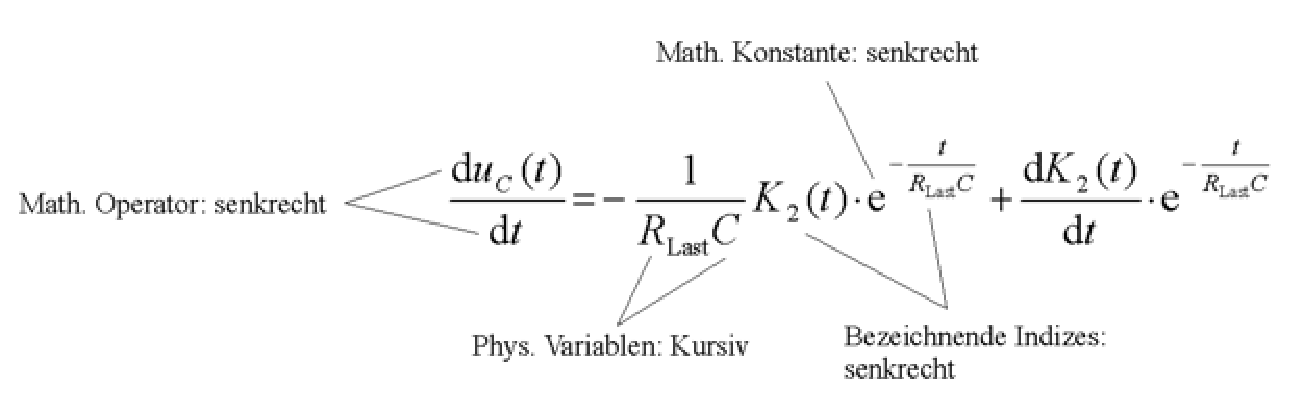
\includegraphics[scale=0.6]{5_Evaluation/formelbeispiel.eps}
				\caption{Formelbeispiel}
				\label{chap2:formelbeispiel}
  		\end{center}
\end{figure}


\begin{table}[!ht]
\caption[In Matlab]{Matlab-Befehle}
\label{tab:ML1}
\begin{tabular}{|| p{7cm} | p{6cm} ||} \hline\hline
I=eye(N);      																									& Einheitsmatrix \\ \hline
e=zeros(N,1); e(j)=1; 																					& Einheitsvektor\\ \hline
D=diag([d11,d22,...,dNN]); 																			& Diagonalmatrix \\ \hline
J=rot90(eye(N)); 																								& Koidentitätsmatrix \\ \hline
E=ones(M,N); 																										& Einsmatrix \\ \hline
eins=ones(N,1); 																								& Einsvektor \\ \hline
t1=[t11,t12,...,t1N]; t2=[t11,t21,...,tN1]; 										& \\
T=toeplitz(t1,t2);  																						& Toeplitzmatrix \\ \hline
t=[t11,t12,...,t1N]; T=toeplitz(t); 														& symmetrische Toeplitzmatrix \\ \hline
x=[x1,x2,...,xN]; v=rot90(vander(x))'; 													& Vandermonde-Matrix \\ \hline
L=tril(A); 																											& untere Dreiecksmatrix der Matrix A \\ \hline
U=triu(A); 																											& obere Dreiecksmatrix der Matrix A \\ \hline\hline
\end{tabular}
\end{table}